\newpage
\fancyhead[LH]{上海交通大学学位论文}
\fancyhead[RH]{第一章\quad 绪论}
\pagenumbering{arabic}
\section{绪论}

\subsection{研究背景与研究意义}

“十三五”期间我国综合交通运输发展取得了显著成效,但与经济社会高质量发展的总体要求相比,仍存在智慧交通发展水平不高、交通基础设施数字化建设亟待加快、交通运输与新技术的融合尚不充分等问题,距离交通强国建设尚有一定差距。随着北斗三号全球卫星导航系统等核心空间基础设施的开通服务、新一代信息技术的发展,构建自主可信、国际领先的时空综合服务体系具备基本条件。2022国家重点研发计划《广域交通可信导航信号与时空服务系统关键技术》应运而生。本课题主要的研究内容响应了该项目的课题3“高精泛源时空感知网络及车路一体化信息融合技术”。

在自动驾驶的落地过程中,车路一体化系统是尤为重要的一环。车路一体化是指利用无线网络,将车端与路端紧密相连,实现车端与路端的信息交换、信息共享。目前,车辆终端导航定位主要依赖于全球卫星导航系统(GNSS),但该系统受限于卫星相关误差、传播途径相关误差、接收机相关误差等限制,对车辆的定位、测速精度有限。以GPS为例,近年来,其定位精度(水平,圆概率精度,CEP)达到了2~3米,其测速精度达到了0.2 m/sec (95\% 置信度)。路侧终端由于可以预先铺设,其位置,硬件设备都是预先获得精确信息的。且路侧终端由于视野开阔,硬件资源丰富,计算能力强大,可以很好的解决车端对自身定位能力不足的问题

我们希望在路边设置一种新型路侧单元,利用激光雷达与相机作为传感器对路过车辆进行定位。将定位结果发送回车端,结合车端GNSS定位结果,基于优化方法,预测车辆位置,最终实现导航增强的功能。本课题对卫星导航脆弱场景下的车辆安全具有重要意义。

\subsection{国内外研究现状}

\subsubsection{车路协同研究现状}

车路协同技术是通过无线通讯技术将车端、路端有机结合起来,实现交通环境数据信息的交换共享,信息处理,从而可以为车辆提供更精确的感知环境信息。

1950年代末,通用汽车在新泽西州打造了一条埋入大量通信设备的高速公路。这在当时引起轰动,也是车路协同产业发展的雏形。加州PATH计划(Partner for Advanced Transit and Highways)成立于1986 年,由加州交通部和加州大学伯克利分校合作建立,是北美第一个专注于现在称为智能交通系统(Intelligent Transportation Systems, ITS)主题的组织。其目标是应用电子、通信与自动化等新兴先进科技,增加高速公路的容量与安全性,减少交通堵塞、空气污染和能源消耗。该计划一直参与自动化公路与自动驾驶车辆的研究、发展与测试之中。被连接的车辆可以与其他车辆或者交通设施,如交通信号灯,进行通信。\cite{xinyanan2022}

车用无线通信技术(Vehicle to Everything, V2X)是将车辆与一切事物相连接的新一代信息通信技术,其中V代表车辆,X代表任何与车交互信息的对象,当前X主要包含车、人、交通路侧基础设施和网络。借助人,车,路,云平台的全方位连接与信息交互,V2X可以提升行驶安全,提高交通效率,提供出行信息服务,支持实现自动驾驶等等。大约在2016年前后,美国基于DSRC(Dedicated Short Range Communications)的V2X协议栈基本制定完毕,并有丰田、通用先后量产支持DSRC的汽车。2022年12月13日,代表整个美国智能交通行业的十大组织联合发出声明,重申了对快速部署V2X的支持,并认为2023年是V2X部署的关键年。

我国工信部早在2018年就明确将5920MHz-5925MHz划分给C-V2X(Cellular Vehicle-to-Everything)并明确表明C-V2X是我国唯一使用的技术路线。2020年发改委联合工信部等其他10个单位发布了《智能汽车创新发展战略》,提到“结合5G商用部署,推动5G与车联网协同建设;开展特定区域智能汽车测试运行及示范应用,验证车辆“人-车-路-云”系统协同性等,支持优势地区创建国家车联网先导区”。

\subsubsection{激光雷达目标跟踪研究现状}

三维激光雷达是一种主动探测式传感器,它向外发出激光束,返回探测到物体的点云数据信息,从而精确地获得探测到物体的距离信息。激光雷达目标跟踪往往是采用基于检测的跟踪范式进行的,其步骤可以大致划分为目标检测,状态预测,数据关联,状态更新共四个部分。其中,目标检测往往用现有的SOTA(state of the art)业界最前沿检测器。状态预测往往用平滑和与滤波方法,根据当前帧的目标的运动状态与位姿,预测下一帧中目标的运动状态与位姿。数据关联将预测的状态值与检测的目标状态匹配在一起,是最重要的步骤。状态更新则根据数据关联的结果,对当前帧目标的运动状态与位姿进行更新。

在目标检测阶段,国内外基于神经网络贡献了不少优秀的算法与思路,按照思路可以分为基于点云的方法,基于体素的方法,基于截面图的方法。\cite{mao20223d}

基于点云的方法直接输入点云进行目标分类分割任务。由于点云是三维不规律信息,典型的卷积网络不方便对点云直接处理。过去的方法大多是划分为规律的空间网格,或者投影到某一截面,从而利用卷积网络处理。但这样将引入冗余信息,并损害原始数据的自然特征。2017年,Charles R. Qi的团队提出了PointNet网络\cite{qi2017pointnet},直接处理点云,考虑到了点云的无序性、空间相关性与旋转不变性。用空间变换网络(spatial transformer network)将点云正则化预处理,也即在空间中旋转对齐。用多层感知机(MLP)将数据从低维投射到高维,避免池化操作中信息损失过多。再用对称性的Max池化函数解决点云输入的无序性,提取出一个高维向量作为全局特征,以此为基础进行后续的分割分类。同年,该团队还提出PointNet++网络\cite{qi2017pointnet++},在PointNet的基础上,进一步考虑了点云的局部信息。首先,利用最远点采样法(FPS)对整个点云进行局部采样,选出若干个中心点。再为每个中心点在一定半径的局部区域内选择k个临近点。最后对每一个局部区域都用PointNet提取局部特征,并以此为基础进行后续的分割分类任务。2019 年,香港中文大学的Shi S团队提出了PointRCNN模型\cite{shi2019pointrcnn},该模型是首个两阶段的基于点云的网络。在第一阶段,模型将整个场景分割为前景点与背景点,对前景点特征提取后生成预选框。在第二阶段通过置信度预测与预选框优化获得最终的检测结果。

基于截面图的方法的代表作是Chen X等人在2017年提出的MV3DNet模型\cite{chen2017multi},该模型同时融合了点云的剖视图特征与RGB图片特征,分别在点云的俯视图、前视图与RGB图像中提取特征。在俯视图特征中计算候选区域后投影到前视图和图像中,经过兴趣区域(ROI)整合到同一纬度再输入网络中融合。

基于体素的方法的代表作是2018年Y. Zhou等人提出的VoxelNet模型\cite{zhou2018voxelnet}。首先将点云划分为等间距的3D体素,经过了点的随机采样与归一化处理后,又引入了体素特征编码器(Voxel Featured Encoding, VFR),每个非空体素都进行了特征提取。然后,这些特征被输入3D卷积神经网络(Convolutional Middle Layers)进行特征抽象。最后通过提议区域生成网络(Region Proposal Network,RPN)进行目标检测。

在数据关联步骤中,常见的算法有全局最近邻法(Global Nearest Neighbor, GNN)、 多 假 设 跟 踪 算 法 (Multiple Hypothesis Tracking, MHT)、联合概率数据关联(Joint Probability Data Association, JPDA)等,该方案的目标匹配精度高,但匹配速度慢、计算成本高。2020 年,Weng X 等人提出了AB3DMOT算法\cite{weng2020ab3dmot} \cite{weng20203d},该算法将匈牙利匹配算法与卡尔曼滤波估计结合,实现了快速的目标关联。

\subsubsection{视觉目标跟踪研究现状}

单目视觉跟踪早期主要采用传统的滤波方法,如卡尔曼滤波(Kalman Filter)、粒子滤波(Particle Filter)、均值漂移(Meanshift)等。近年来流行的研究框架可以分为相关滤波(Correlation Filter)框架与孪生网络(Siamese Network)框架两个大方向。

2010年,Bolme团队首次将相关滤波方法用在了跟踪领域,提出了误差最小平方和滤波器(Minimum Output Sum of Squared Error filter, MOSSE)\cite{bolme2010visual},用最小化均方误差的思路产生滤波器,进而获得跟踪目标的新位置。2012年,Henriques等人在MOSSE的基础上提出了循环结构检测方法(Circulant Structure with Kernal)\cite{henriques2012exploiting},一方面修改损失函数为岭回归形式,再引入核函数求解,另一方面引入循环矩阵,达到密集采样与提高运算效率的效果。2014年,Henriques等人提出了核相关滤波算法(Kernel Correlation Filter, KCF)\cite{henriques2014high},该方法在CSK算法的基础上,用方向梯度直方图(Histogram of Oriented Gradient,HOG)多通道特征替换了原来的单通道灰度特征,并采用了高斯核函数求解岭回归问题。同一年,Danelljan等人提出了DSST(Discriminative Scale Space Tracker)\cite{danelljan2015convolutional}方法,在MOSSE的基础上,用两个滤波器分别应对尺度和位置的变化,同时引入HOG特征。

孪生网络框架,采用两个成对的结构一样的神经网络,网络之间共享权值、参数等信息。该框架可以接受两个输入,并对两个输入进行相同的变换,通过比较输出的两个结果的欧氏距离判断输入之间的相似性。这一思路最早在1993年被J Bromley应用在美国支票的签名验证场景上\cite{bromley1993signature}。在目标跟踪问题里,一个输入可以是初始帧的目标区域,以此作为模板,而将后一帧中的候选区域作为第二个输入。孪生网络要做的就是找到两帧间相似度最高的候选区域,如这一系列的开山之作SiamFC框架\cite{bertinetto2016fully}。

\subsubsection{激光雷达与视觉融合研究现状}

传感器信息融合可以分为像素级、特征级和目标级融合\cite{wang2020jiyusanweileida}。像素级融合直接融合原始数据,获取的细节信息最丰富,因而其准确性和鲁棒性最好。但是像素级融合的前提是信息来自于同类传感器或者传感器拥有同样的量级,需要传感器之间进行高精度匹配,因而实时性较低。特征级融合先提取原始数据的特征,再融合多个特征,根据目标已有特征对融合特征进行匹配,获得目标的信息。目标级融合先提取原始数据中的目标信息,然后融合多个目标信息,得到最终完整信息。其只对目标信息进行融合,不受传感器类别的限制,能够保证实时性。

EagarMOT是Aleksandr Kim等人2021年提出的融合框架\cite{kim2021eagermot},用现成的2D与3D检测器先得到目标的2D与3D检测结果,再用交比IoU将同一个目标的两个结果关联在一起得到一个融合实例。在数据关联部分,该方法采用两阶段进行,第一阶段对3D检测结果和预测结果进行数据关联,对于没有匹配上的实例和轨迹再进入第二阶段匹配,利用2D检测结果进行数据关联。

\subsection{研究内容与研究路线}

\subsubsection{研究路线}

我们希望在路边设置一种新型路侧单元,上面装备了相机、激光雷达等传感器。利用激光雷达的测距测向功能获得深度信息,利用相机的色彩捕捉功能获得图像信息,通过2d-3d融合的多目标跟踪方法,获得车辆相对路侧传感器的相对位置姿态。然后,通过路侧与车端的可靠通信,将位姿传回车端,车端利用其作为新增的独立位置约束,结合误差检测与估计理论,提高车辆当前位置估计的精确度,提高车辆导航的可信性。如下图所示:

\begin{figure}[htb] 
    \center{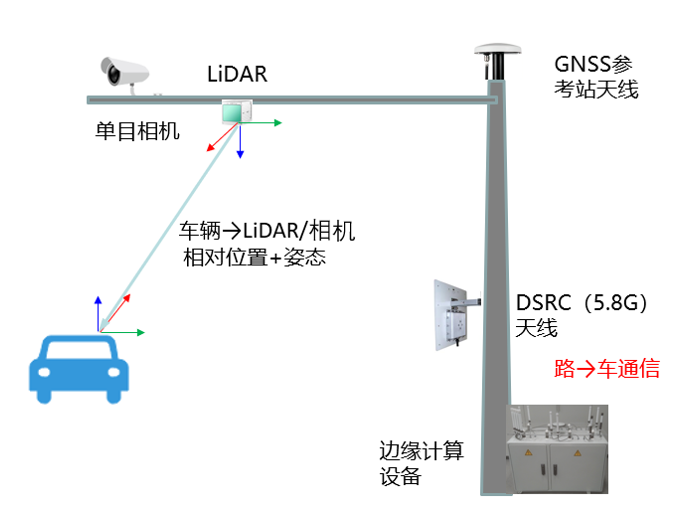
\includegraphics[width=0.7\textwidth]  {figure/fig3.png}} 
    \caption{路侧单元架设示意图}
\end{figure}

但受到实验条件限制,目前硬件平台尚未搭建完全,作者也身处国外,所以只能依托公开数据集进行实验。

\subsubsection{研究内容}

本文主要依托现有公开数据集,搭建了目标跟踪器,训练了二维与三维检测器,并提出了一种基于因子图的误差补偿方法。本文主要内容如下所示:

第一章为绪论。对本课题的研究背景与意义进行论述,回顾了车路一体化概念的发展历史,对众多国内外基于激光雷达和基于视觉的目标跟踪方法进行阐述,分析了国内外基于传感器融合的目标跟踪方法,并确定了本文的研究路线。

第二章为现有公开数据集框架。首先总结了近年来适用于自动驾驶与车路协同的公开数据集。再介绍了KITTI数据集和DAIR-V2X数据集的传感器配置,标签与标定格式,其中包括了激光雷达与摄像头的标定原理及其坐标转换关系。

第三章为目标跟踪器搭建。首先介绍了EagerMOT目标跟踪框架的原理,再介绍了目标跟踪常用的评测方法,最后在KITTI数据集上复现了该框架,并与论文结果进行了对比。

第四章为目标检测器训练。首先介绍了2D检测器YOLOv4的原理,训练环境与网络配置,训练结果。再介绍了3D检测器PointRCNN的原理,训练环境与网络配置,训练结果。最后对检测器训练结果进行了分析。

第五章为基于优化的路侧导航增强原理,首先介绍了基于因子图的优化方法,再针对本课题场景提出了路侧导航增强原理。

第六章为总结与展望,首先总结本文的主要工作,然后展望后续的研究与改进工作。

\subsection{本章小结}

本章介绍了研究背景与意义,国内外研究现状,研究内容与研究路线。